\documentclass{beamer}
\usepackage[utf8]{inputenc}
\usepackage{remreset}
\usepackage{tikz}

\usetheme{Frankfurt}
\setbeamertemplate{navigation symbols}{}

\usetikzlibrary{shapes}

\makeatletter
\@removefromreset{subsection}{section}
\makeatother
\setcounter{subsection}{1}

\title{\textbf{Conductor} \\
	An automatic audio routing system based on \\
	the RSSI of a passive Bluetooth device}
\author{Davide Pesavento \and Martina Astegno}
\institute{Università degli Studi di Padova \\
	Corso di Laurea Magistrale in Informatica}
\date{\today}

\renewcommand{\baselinestretch}{1.2}


\begin{document}

\begin{frame}[plain]
\titlepage
\end{frame}

\begin{frame}
\frametitle{Outline}
\tableofcontents
\end{frame}

%_____________________%

\section[Introduction]{Introduction: goals and requirements}

\begin{frame}
\frametitle{Project's goals}
\setbeamercovered{transparent}
\begin{enumerate}
	\pause
	\item \textbf{Locating} a person wearing a Bluetooth device among a predefined set of rooms.
	\pause\vspace{1cm}
	\item \textbf{Redirecting} the output of an audio player from one room to another, according to the person's movements.
\end{enumerate}
\setbeamercovered{invisible}
\end{frame}

\begin{frame}
\frametitle{Required setup}
Globally:
\begin{itemize}
	\item a Bluetooth-equipped \textbf{device}, used to track the person's movements across rooms;
	\item a \textbf{central server}, where the audio player and the main \textsl{Conductor} application run.
\end{itemize}
\vspace{3mm}
And for each room:
\begin{itemize}
	\item one Bluetooth \textbf{adapter}, for device discovery and monitoring;
	\item one \textbf{speaker}, for sound playback.
\end{itemize}
\end{frame}

\begin{frame}
\frametitle{Employed technologies}
\begin{center}
{\large Short-range device discovery $\Rightarrow$ \textbf{BlueZ}} \\\vspace{2mm}
{\footnotesize the official Linux Bluetooth stack implementation,\\exposes an easy-to-use DBus interface}
\\\pause\vspace{1cm}
{\large Audio routing $\Rightarrow$ \textbf{PulseAudio}} \\\vspace{2mm}
{\footnotesize a cross-platform, networked sound server that allows\\to perform advanced operations on audio data}
\end{center}
\end{frame}

%_____________________%

\section[Prototype design]{Prototype design: Bluetooth and PulseAudio components}

\begin{frame}
\frametitle{Bluetooth component}
The Bluetooth component deals with the discovery and monitoring of the mobile device.
\begin{itemize}
	\item It relies on \textbf{Probe}, a simple CLI application.
	\begin{itemize}
		\item one instance for each Bluetooth adapter
		\item basically a proxy between \textsl{Conductor} and the adapters
		\item \textbf{DBus} is used to interface with the BlueZ daemon
	\end{itemize}
	\item It controls all BT operations via the \texttt{ProbeManager} class.
	\begin{itemize}
		\item it connects to all available \textsl{Probe}s upon startup
		\item it sends them commands to start or stop a discovery session
		\item it emits a signal when the RSSI detected by a \textsl{Probe} changes
	\end{itemize}
\end{itemize}
\end{frame}

\begin{frame}
\frametitle{PulseAudio component}
Three main responsibilities:
\begin{enumerate}
	\item \textbf{querying} the daemon for the list of sinks and streams;
	\item \textbf{loading/unloading} PulseAudio modules;
	\item \textbf{redirecting} an audio stream from one sink to another.
\end{enumerate}
\pause\vspace{3mm}
Each operation is wrapped by a subclass of \texttt{PAOperation}, e.g.:
\begin{itemize}
	\item \texttt{LoadModuleOperation}: loads one of the following modules:
	\begin{description}
		\item[\texttt{module-tunnel-sink}] $\rightarrow$ creates a virtual sink that forwards its input to a remote PulseAudio instance
		\item[\texttt{module-combine}] $\rightarrow$ allows playing the same stream through two or more sinks simultaneously
	\end{description}
	\item \texttt{MoveOperation}: performs stream redirection.
\end{itemize}
\end{frame}

\begin{frame}
\frametitle{General architecture}
\begin{center}
\begin{tikzpicture}
	[e/.style={red,very thick}]
	\node[anchor=south west,inner sep=0] at (0, 0)	{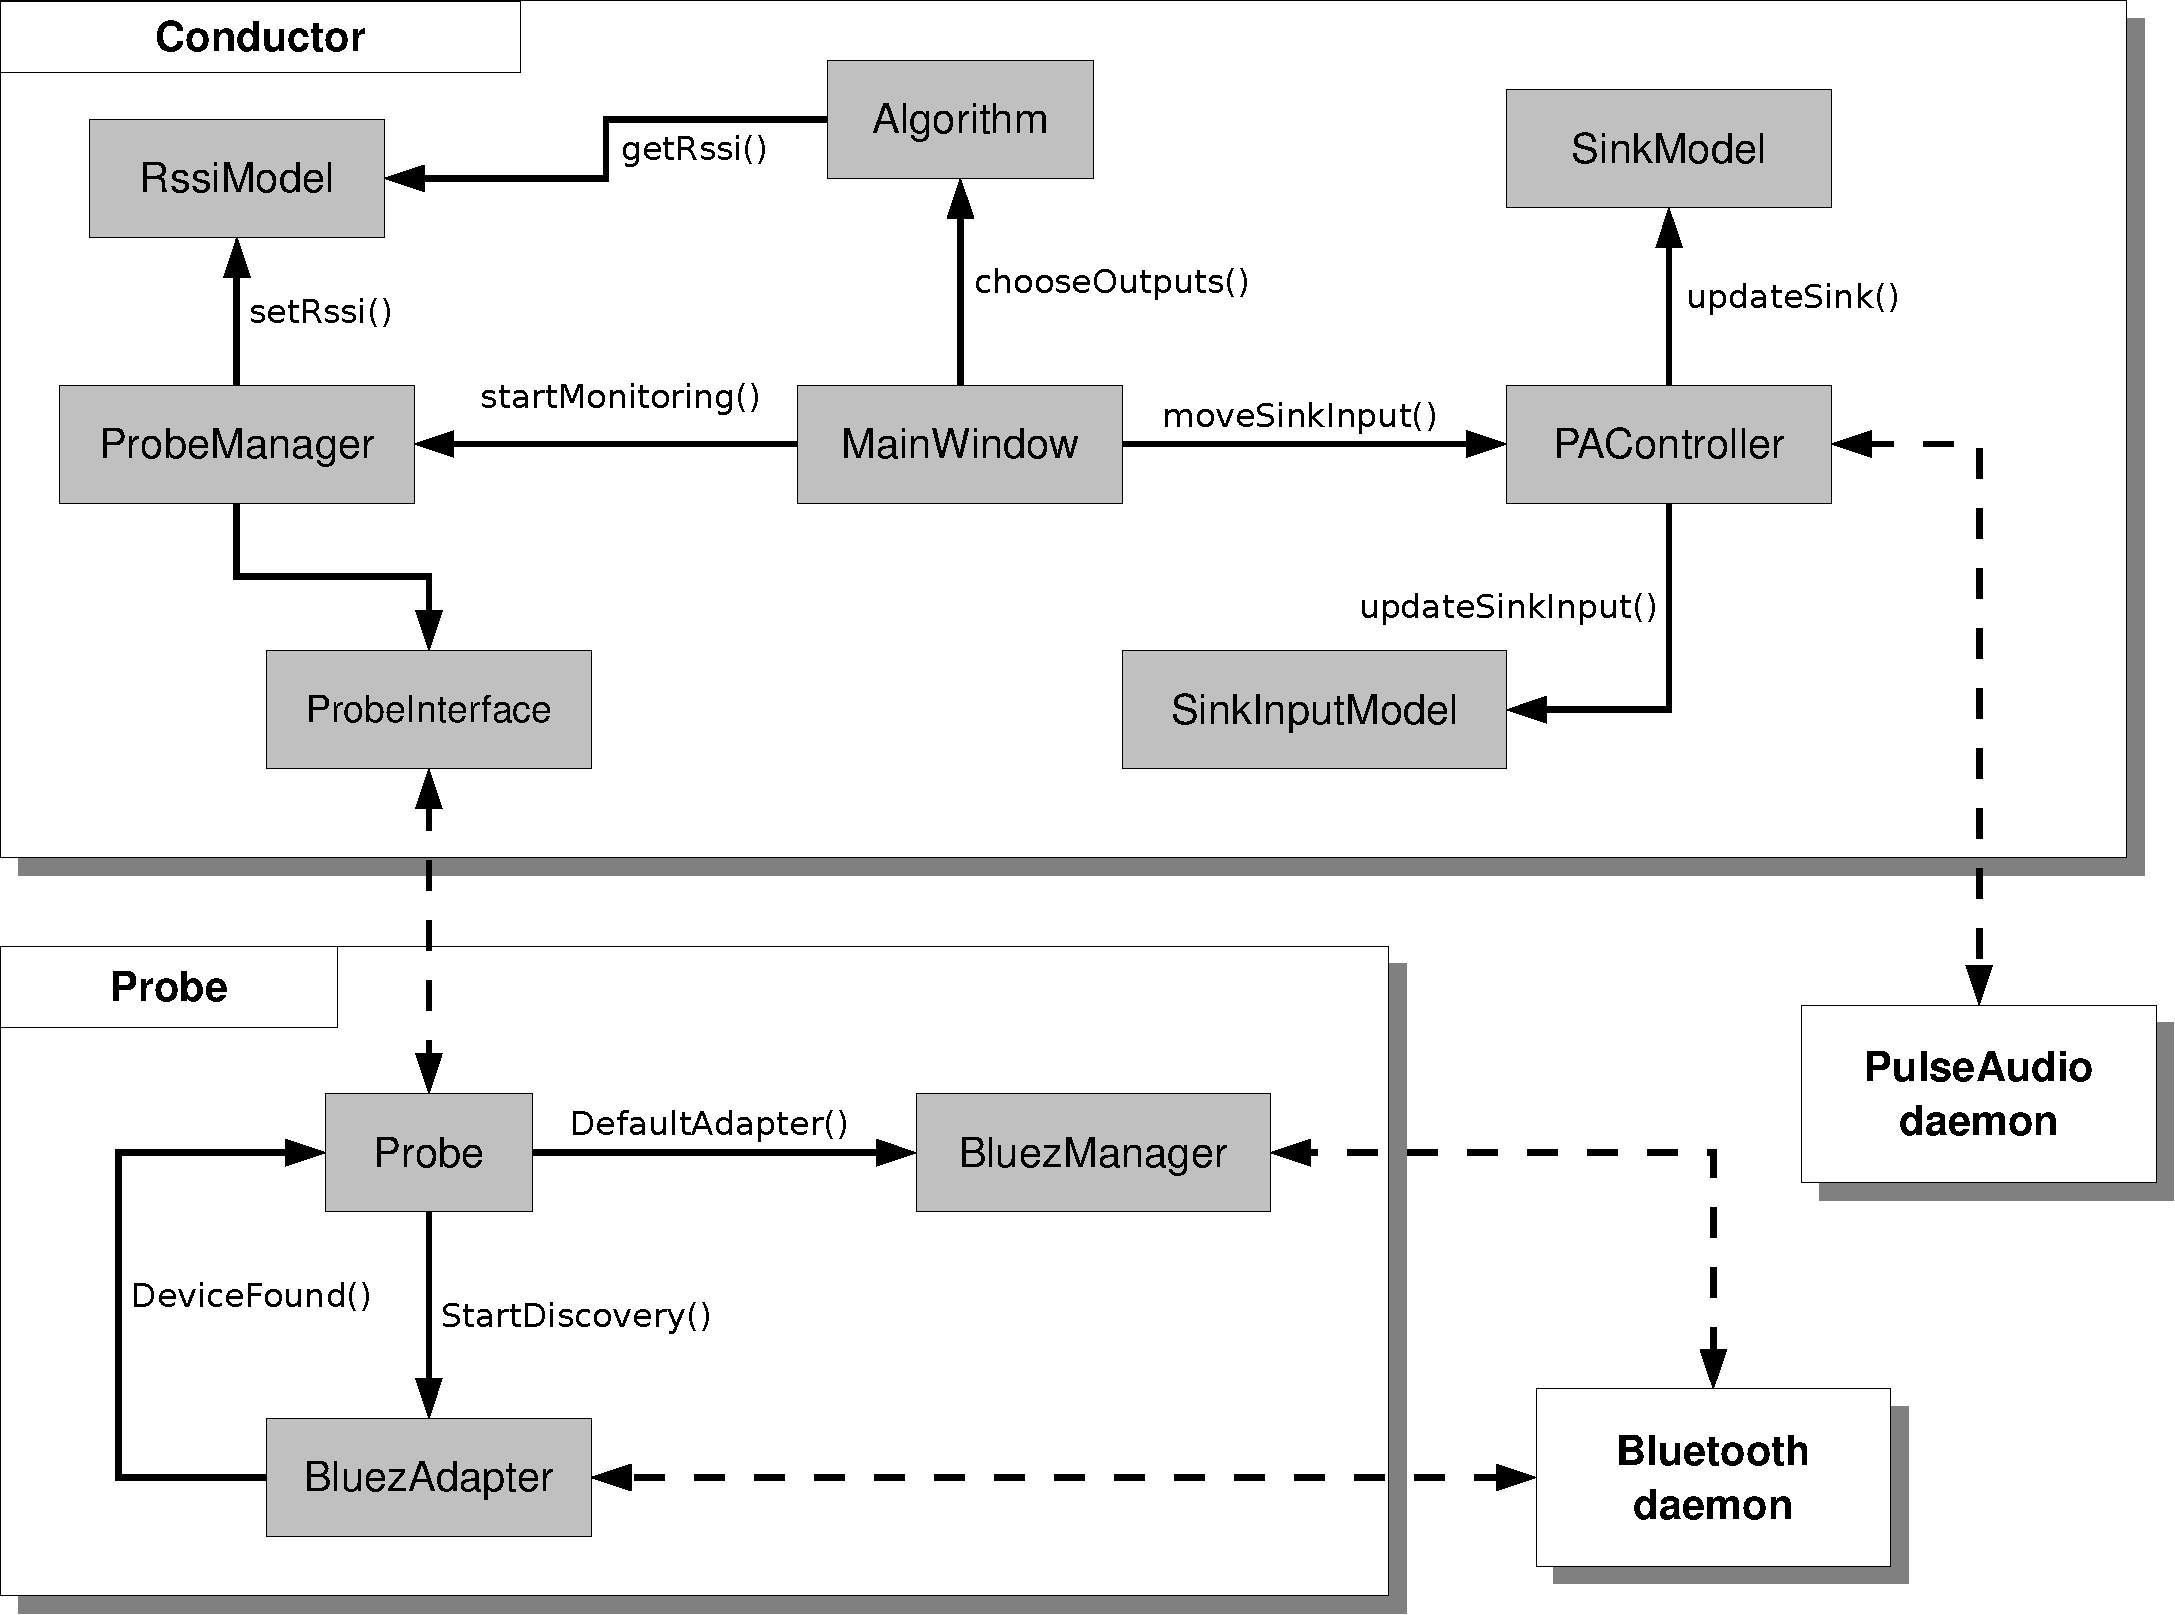
\includegraphics[scale=.25]{Arch}};
	\onslide<2>
	\draw[e]	(2.6, 5.16)	ellipse[x radius=8mm, y radius=2.5mm]
			(2.45, 1.26)	ellipse[x radius=8mm, y radius=2.5mm];
	\onslide<3>
	\draw[e]	(1.05, 1.38)	ellipse[x radius=7mm, y radius=2.5mm];
	\onslide<4>
	\draw[e]	(1.35, 5.52)	ellipse[x radius=6.5mm, y radius=2mm];
	\onslide<5>
	\draw[e]	(4.15, 6.1)	ellipse[x radius=18mm, y radius=8mm];
	\onslide<6>
	\draw[e]	(5.52, 5.08)	ellipse[x radius=7.5mm, y radius=2.5mm];
	\onslide<7>
\end{tikzpicture}
\end{center}
\end{frame}

%______________________%

\section{Possible extensions}

\begin{frame}
\frametitle{Future extensions}
\begin{itemize}
	\item \textbf{Testbed improvements:} the prototype has only been tested in a simulated environment. It would be interesting to perform a more thorough testing session in a real-world scenario.
	\pause
	\item \textbf{Multiple monitored devices:} adding support for more than one device would be a major feature. This entails the necessity of evaluating how different devices could interact.
	\pause
	\item \textbf{Control application:} develop a mobile application that allows the end user to control audio streams, e.g.\ adjusting the volume, pausing, managing the playlist, \ldots
\end{itemize}
\end{frame}

%______________________%

\section{Conclusions}

\begin{frame}
\frametitle{Issues experienced}
\begin{itemize}
	\item Available Bluetooth hardware was unsuitable, it did not satisfy needed requirements.
	\pause
	\item PulseAudio is not fully reliable when tunneling and moving streams (excessive latency, incorrect resampling).
	\pause
	\item All PulseAudio operations are executed asynchronously, it has been difficult to properly handle them.
\end{itemize}
\end{frame}

\begin{frame}
\frametitle{Final considerations}
\begin{itemize}
	\item Bluetooth: very low power consumption, but high variance in reported RSSI values.
	\item PulseAudio: quite advanced and featureful, but some areas need more polishing.
	\item Prototype: overall it is a good starting point for future extensions and improvements.
\end{itemize}
\end{frame}

%______________________%

\appendix

\begin{frame}
\frametitle{References}
\begin{itemize}
	\item[$\vartriangleright$] \textbf{BlueZ: the official Linux Bluetooth protocol stack} \\
			{\footnotesize\url{http://www.bluez.org/}}
	\item[$\vartriangleright$] Marcel~Holtmann, \textbf{Playing BlueZ on the D-Bus} \\
			{\footnotesize\url{www.kernel.org/doc/ols/2006/ols2006v1-pages-421-426.pdf}}
	\item[$\vartriangleright$] \textbf{PulseAudio sound server} \\
			{\footnotesize\url{http://www.pulseaudio.org/}}
	\item[$\vartriangleright$] \textbf{PulseAudio API documentation} \\
			{\footnotesize\url{http://0pointer.de/lennart/projects/pulseaudio/doxygen/}}
\end{itemize}
\end{frame}

\end{document}
